\documentclass[mathserif,9pt]{beamer}
%\documentclass{article}



%\usepackage{beamerarticle}

\mode<presentation>
{
\usetheme{Rob}
\beamertemplatenavigationsymbolsempty
}

\usepackage{thumbpdf}
\usepackage{wasysym}
%\usepackage{ucs}
\usepackage[utf8]{inputenc}
\usepackage{pgf,pgfarrows,pgfnodes,pgfautomata,pgfheaps,pgfshade}
\usepackage{pstricks,pst-node, pst-tree}
\usepackage{verbatim,bm}


\usepackage{xcolor,eurosym}

\DeclareMathOperator{\maximize}{maximize}
\DeclareMathOperator*{\argmin}{arg\,min}
\DeclareMathOperator{\E}{\mathbb{E}}
\DeclareMathOperator{\V}{\mathbb{V}}
\DeclareMathOperator{\COV}{\mathbb{COV}}
\newcommand{\bs}{\boldsymbol}
\newcommand{\dd}{\mathrm{d}}
\newcommand{\pkg}[1]{{\normalfont\fontseries{b}\selectfont #1}}
\let\proglang=\textsf


\definecolor{craneblue}{RGB}{255,76,0}
\setbeamercolor{alerted text}{fg=craneblue}

\pdfinfo
{
  /Title       (Dynamic Estimation of the Zero-Coupon Yield Curve)
  /Creator     (LaTeX)
  /Author      (Robert Ferstl, Josef Hayden)
}


\title{Generation Capacity Investment in Oligopolistic Electricity Markets under Uncertainty}
\subtitle{\scriptsize\vspace{0.2cm}ISBIS-2008 International Symposium on Business and Industrial Statistics\\\vspace{0.2cm}\em Prague, Czech Republic}
%\author{Robert Ferstl}

\author[Anton Burger\and Robert Ferstl]{Anton Burger\inst{1} \and Robert Ferstl\inst{1}}


\institute[Universities Vienna and Regensburg]{
\inst{1}Research Institute for Regulatory Economics\\
Vienna University of Economics and Business Administration, Austria
\and
\inst{2}Department of Finance\\
University of Regensburg, Germany}

\date{July 1-4, 2008}

\begin{document}

\frame{\titlepage}

\section*{}
 \begin{frame}
   \frametitle{Outline}
   \tableofcontents[section=1,hidesubsections]
 \end{frame}

%  \AtBeginSection[]
%  {
%    \frame<handout:0>
%    {
%      \frametitle{Outline}
%      \tableofcontents[currentsection,hideallsubsections]
%    }
%  }

%  \AtBeginSubsection[]
%  {
%    \frame<handout:0>
%    {
%      \frametitle{Outline}
%      \tableofcontents[sectionstyle=show/hide,subsectionstyle=show/shaded/hide]
%    }
%  }

\newcommand<>{\highlighton}[1]{%
  \alt#2{\structure{#1}}{{#1}}
}

\newcommand{\icon}[1]{\pgfimage[height=1em]{#1}}



%%%%%%%%%%%%%%%%%%%%%%%%%%%%%%%%%%%%%%%%%
%%%%%%%%%% Content starts here %%%%%%%%%%
%%%%%%%%%%%%%%%%%%%%%%%%%%%%%%%%%%%%%%%%%

\section{Motivation}

\begin{frame}
  \frametitle{Motivation}
  \begin{itemize}
  \item \euro\euro\euro
  \item dynamic forecast of zero-coupon yield curves
  \item useful for bond portfolio management, hedging interest rate risk, identify arbitrage opportunities, ...
  \item further step towards arbitrage-free model with joint estimation procedure
  \end{itemize}
\end{frame}


\section{Motivation}

\begin{frame}{Motivation}

\begin{itemize}
	\item electricity markets are liberalized
	\item profit maximizing players instead of central capacity planning 
	\item \textbf{decentralized} market decisions
\end{itemize}	

there are qualms about adequacy of investments
	
\begin{itemize}
	\item California blackouts
	\item nuclear phase out in Germany
	\item aging capacities throughout Europe and the US
\end{itemize}

\end{frame}

\section{Multistage Model}
%\subsection{Overview}

\begin{frame}{Multistage Model}
  \begin{itemize}
  \item stochastic dynamic equilibrium model
  \item long-run economic effects of strategic investment decisions
  \item oligopolistic market structure
  \end{itemize}
  \begin{itemize}
  \item multi-stage stochastic program with recourse
  \item uncertainty is reflected in future level of demand and strategic investment decisions 
  \item solution as mixed complementarity problem (MCP) with GAMS and PATH solver
   \item $S$-adapted open-loop information structure leads to Nash equilibria in each node 
  \end{itemize}
\end{frame}



%\subsection{Scenario Tree}

\begin{frame}{Scenario Tree}
\begin{center}
\psscalebox{0.60}{
\psset{nodesep=0pt,labelsep=1pt,nrot=:U}
\psmatrix[colsep=3.0cm,rowsep=0.0cm] 
                               &                                    &                                       & \circlenode{H}{$n_7$}\\ 
                               &                                    & \circlenode{D}{$n_3$}\\  
                               &                                    &                                       & \circlenode{I}{$n_8$}\\              
                               &  \circlenode{B}{$n_1$} & & \\
                               &                                    &                                       & \circlenode{J}{$n_9$}\\ 
                               &                                    & \circlenode{E}{$n_4$}\\  
                               &                                    &                                       & \circlenode{K}{$n_{10}$}\\ 
    \circlenode{A}{$n_0$} &                          &              & \\
                               &                                    &                                       & \circlenode{L}{$n_{11}$}\\ 
                               &                                    & \circlenode{F}{$n_5$}\\  
                               &                                    &                                       & \circlenode{M}{$n_{12}$}\\              
                               &  \circlenode{C}{$n_2$} & & \\
                               &                                    &                                       & \circlenode{N}{$n_{13}$}\\ 
                               &                                    & \circlenode{G}{$n_6$}\\  
                               &                                    &                                       & \circlenode{O}{$n_{14}$}\\ 
& & & \\
 $t=0$ & $t = 1$ & $t=2$ &  $t=3$\\
\ncline[linewidth=1.5pt]{A}{B}\naput{$50\%$}
\ncline[linewidth=1.5pt]{A}{C}\naput{$50\%$}
\ncline[linewidth=1.5pt]{B}{D}\naput{$25\%$}
\ncline[linewidth=1.5pt]{B}{E}\naput{$25\%$}
\ncline[linewidth=1.5pt]{C}{F}\naput{$25\%$}
\ncline[linewidth=1.5pt]{C}{G}\naput{$25\%$}
\ncline[linewidth=1.5pt]{D}{H}\naput{$12.5\%$}
\ncline[linewidth=1.5pt]{D}{I}\naput{$12.5\%$}
\ncline[linewidth=1.5pt]{E}{J}\naput{$12.5\%$}
\ncline[linewidth=1.5pt]{E}{K}\naput{$12.5\%$}
\ncline[linewidth=1.5pt]{F}{L}\naput{$12.5\%$}
\ncline[linewidth=1.5pt]{F}{M}\naput{$12.5\%$}
\ncline[linewidth=1.5pt]{G}{N}\naput{$12.5\%$}
\ncline[linewidth=1.5pt]{G}{O}\naput{$12.5\%$}
\endpsmatrix}
\end{center}
\end{frame}


\begin{frame}{Notation}
  \begin{tabular}[l]{l l}
\centering
$i \in \mathcal{I}$ & players, firms \\
$j \in \mathcal{J}$ & available technologies \\
$m\in\mathcal{M}$ & market states \\
$p_n$ & probability to reach a certain node\\
$p^m$ & probability of market state $m$ \\
$ q_{i,n}^{j,m}$ & production quantities \\
$I_{i,n}^{j}$ & investment quantities, for $n\in\left\{n_0\right\}\cup\mathcal{T}$ \\
$K_{i,n}^{j}$ & available capacity\\
$F_n^{j}$ & investment cost\\
$P^m_n = \alpha_n^m-\beta^m\sum_{i\in \mathcal{I}}\sum_{j\in \mathcal{J}}q_{i,n}^{j,m}$ & market equilibrium price \\
$\alpha_n^m$ & intercept of demand function \\
$\beta^m$ & slope of demand function \\
$c_j$ & variable costs \\
$\delta_n$ & discount factor \\
$\nu$ & salvage value parameter\\
$\rho$ & depreciation rate\\
\end{tabular}
\end{frame}

\begin{frame}{Optimization Problem}

\begin{equation*}
  \label{eq:objfct}
  \max_{q_{i,n}^{j,m}, I_{i,n}^{j}} \sum_{n\in \mathcal{N}}p_n\delta_n\Pi_{i,n}\left(q_{i,n}^{j,m}, I_{i,n}^{j}, K_{i,n}^{j}, Q_n^m\right)+ \sum_{n\in \mathcal{S}}p_n\,\delta_n \sum_{j\in \mathcal{J}}K_{i,n}^{j}F_n^{j}\nu
\end{equation*}
subject to
  
\begin{eqnarray*}  
q_{i,n}^{j,m} - K_{i,n}^{j} &\leq& 0 \quad \forall i,j,m,n \label{eq:prodconstr} \\
Q_n^m-\sum_{i\in \mathcal{I}}\sum_{j\in \mathcal{J}} q_{i,n}^{j,m} &=& 0 \quad \forall m,n \label{eq:marketclearing}\\
K_{i,n}^{j} - (1-\rho)K_{i,a(n)}^{j}-I_{i,a(n)}^{j} &=& 0 \quad \forall i,j,n \label{eq:state} \\
q_{i,n}^{j,m}, K_{i,n}^{j}, I_{i,n}^{j}, Q_n^m  &\geq& 0 \quad \forall i,j,m,n\label{eq:nonneg}
\end{eqnarray*}
  
\end{frame}

\begin{frame}[allowframebreaks]{KKT Conditions}
  
\begin{align*}
0\leq - p_n\delta_np^m\left(\alpha_n^m-\beta^m Q_n^m-\beta^m\sum_{j^*\in \mathcal{J}}q_{i,n}^{j,m}-c_j\right) \nonumber\\
+\lambda_{i,n}^{1,j,m} &\quad\bot&q_{i,n}^{j,m}\geq 0&  \quad \forall i,j,m,n\label{eq:kkt_first}
\end{align*}

$\lambda_{i,n}^{1,j,m}\dots$ shadow price of of capacity in each market state

\vspace{0.5cm}

\begin{itemize}
  \item expected marginal revenues = expected marginal costs + scarcity rent
\end{itemize}

\begin{center}
\begin{tabular}{ll}
\hline
perfect competition &$\alpha_n^m-\beta^m Q_n^m$ \\
oligopoly & $\alpha_n^m-\beta^m Q_n^m-\beta^m\sum_{j^*\in \mathcal{J}}q_{i,n}^{j,m}$  \\
monopoly   & $\alpha_n^m-2\beta^m Q_n^m$  \\
\hline
\end{tabular}
\end{center}


\begin{itemize}
	\item imperfect competition distorts quantities and thereby investments $\Downarrow$
\end{itemize}

\framebreak

\begin{align*}
  0 \leq -\sum_{m\in\mathcal{M}}\lambda_{i,n}^{1,j,m}  +\phi_{i,n}^{2,j} &\quad\bot&K_{i,n}^{j}\geq 0&  \quad \forall i,j,n\in\mathcal{T}\\
0 \leq -\sum_{m\in\mathcal{M}}\lambda_{i,n}^{1,j,m}  +\phi_{i,n}^{2,j}-p_n\delta_nF_n^j\nu &\quad\bot&K_{i,n}^{j}\geq 0&  \quad \forall i,j,n\in\mathcal{S}\\
0\leq p_n\delta_nF_n^{j} - \sum_{n'\in a(n)}\phi_{i,n'}^{2,j} &\quad\bot&I_{i,n}^{j}\geq 0&  \quad \forall i,j,n\in\mathcal{T}\\
\end{align*}

$\phi_{i,n}^{2,j}\dots$ shadow prices of capacity in all market states

\vspace{0.5cm}

\begin{itemize}
	\item investments until \textbf{marginal profit} equal to \textbf{marginal costs}
	\item real option interpretation - only investments if the expected gain $\geq$ investment costs
\end{itemize}




\end{frame}

\section{The German Electricity Market}

%\subsection{Installed Capacities}

\begin{frame}{Installed Capacities}
					
\begin{figure}[h]
  \centering
%\caption{Installed capacities in GW of major players in Germany}
\includegraphics[width=0.8\textwidth]{capacities}
  \label{fig:capacities}
\\
\vspace{0.1cm}
\scriptsize Source: International Energy Agency (2007)
\end{figure}

\end{frame}

%\subsection{Electricity Load and Prices}

\begin{frame} {Electricity Load}
					
\begin{figure}[h]
\centering
\includegraphics[width=0.9\textwidth, angle=0]{loadvalues}
    \label{fig:load}   
\\ 
\vspace{0.1cm}
\scriptsize Source: UCTE (2006)           
\end{figure}
\end{frame}

\begin{frame} {Electricity Prices}				
\begin{figure}[h]
\centering
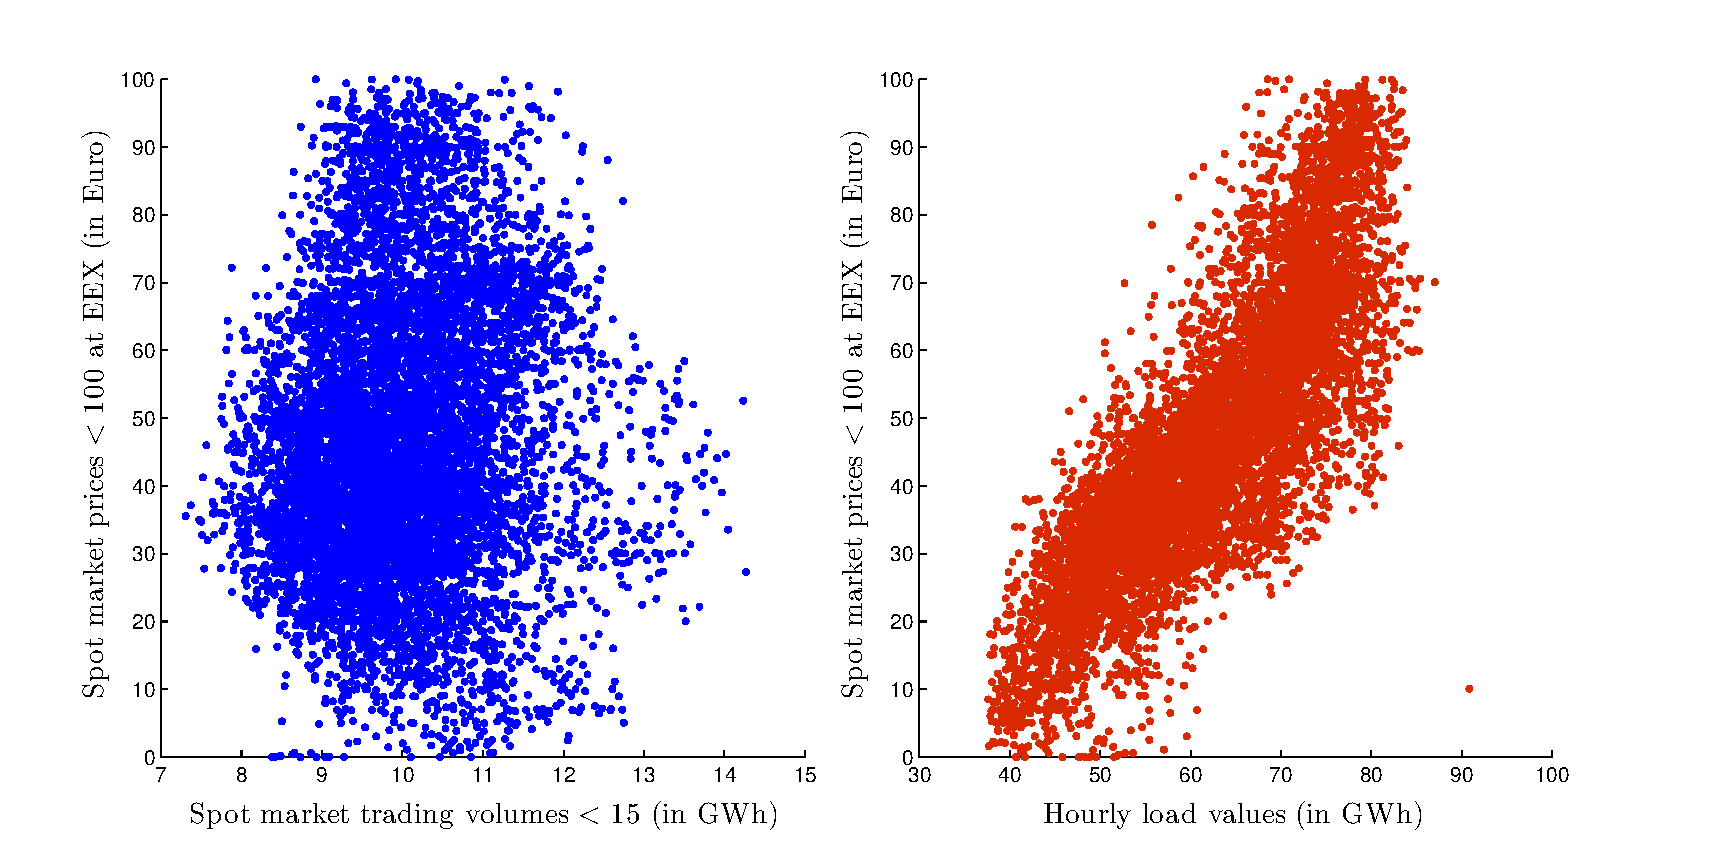
\includegraphics[width=1.0\textwidth, angle=0]{pricequant}
    \label{fig:load} 
\\ 
\vspace{0.1cm}
\scriptsize Source: EEX (2006); UCTE (2006)           
\end{figure}
\end{frame}

\begin{frame}
  \frametitle{Market Segments}

\begin{center}
\small
\begin{tabular}{rrrrr}
  \hline
Price & Average price  & Average quantity & Number of & Percentage of \\
intervals& (Euro/MWh) &  (MWh) &  prices & of total prices\\
  \hline\hline
$0\leq p<20$ & 12.67 & 46,111.63 & 611 & 6.98\% \\
$20\leq p<40$ & 31.35 & 54,103.50 & 3,003 & 34.28\% \\
$40\leq p<60$ & 49.00 & 64,806.04 & 2,626 & 29.98\% \\
$60\leq p<80$ & 68.46 & 72,385.56 & 1,588 & 18.13\% \\
$80\leq p<100$ & 88.40 & 75,991.21 & 665 & 7.59\% \\
$100\leq p<\infty$& 176.06 & 76,482.34 & 266 & 3.04\% \\
   \hline
\end{tabular}  
\normalsize
\end{center}

\end{frame}

%\subsection{Marginal and Investment Costs}

\begin{frame}
  \frametitle{Marginal and Investment Costs}
\begin{center}
  \begin{tabular}{rrr}
\hline
           & Variable costs & Investment costs\\
           &  (Euro/MWh)    &  (Euro/GW) \\
\hline\hline
     Hydro &        7.6 &    3,500\\

   Nuclear &        9.5 &    1,841 \\

   Lignite &       10.6 &    1,074 \\

 Hard coal &       16.1 &     971 \\

 Gas (CCGT) &       33.5 &     460 \\

Oil & 44            &   n/a\\

Pump &         80 &       n/a\\
\hline
\end{tabular}
\\
\vspace{0.3cm}
\scriptsize Source: Auer et al. (2006)
\end{center}
\end{frame}

\section{Results}

%\subsection{Scenario Generation}

\begin{frame}
  \frametitle{Scenario Generation}
\begin{figure}[h]
  \centering
\includegraphics[width=1\textwidth]{intercept}
  \label{fig:intercept}
\end{figure}  
\end{frame}


%\subsection{Solution of the MCP}

\begin{frame}
  \frametitle{Production in the initial node $q_{i,0}^{m}$ (in MWh)}
  \begin{center}
\small
      \begin{tabular}{rrrrrrr}
\hline
           &     $m=1$ &     $m=2$ &     $m=3$ &     $m=4$ &     $m=5$ &     $m=6$ \\
\hline\hline
       Rwe &    10,945.21  &    13,590.03  &    17,150.64  &    20,586.19  &    21,872.07  &    21,984.52  \\

       EON &    10,945.21  &    13,592.14  &    17,150.64  &    20,586.09  &    21,871.99  &    21,984.48  \\

    Vattenfall &    10,940.85  &    13,590.03  &    15,273.00  &    15,273.00  &    15,273.00  &    15,273.00  \\

      EnBW &    10,528.00  &    10,528.00  &    10,528.00  &    10,528.00  &    10,528.00  &    10,528.00  \\
\hline
\end{tabular}
\normalsize
  \end{center}
\end{frame}



\begin{frame}
  \frametitle{Sensitivity Analysis}

  \begin{itemize}
  \item Investment quantities in the initial node $I_{i,0}$ (in MW) with $\rho=0.025$
  \end{itemize}

\begin{center}
  \begin{tabular}{rrrrr}
\hline
           &       $\nu=0.99$ &       $\nu=0.95$ &        $\nu=0.9$ &       $\nu=0.85$ \\
\hline\hline
 Vattenfall  &      5,015.93  &      4,832.23  &      4,626.18  &      4,516.54  \\

     EnBW  &      9,582.64  &      9,405.55  &      9,229.64  &      9,120.00  \\
\hline
\end{tabular}
\end{center}

\begin{itemize}
\item Investment quantities in the initial node $I_{i,0}$ (in MW) with $\nu=0.95$
\end{itemize}

\begin{center}
  \begin{tabular}{rrrrr}
\hline
           &      $\rho=0.025$ &       $\rho=0.03$ &      $\rho=0.035$ &       $\rho=0.04$ \\
\hline\hline
Vattenfall &      4,832.23  &      4,908.60  &      4,984.96  &      5,061.33  \\

      EnBW &      9,405.55  &      9,458.19  &      9,510.83  &      9,563.47  \\
\hline
\end{tabular}  
\end{center}

\end{frame}

\section{Conclusion}
\begin{frame}
  \frametitle{Conclusion}
  \begin{itemize}
  \item generation capacity investment game under uncertainty
  \item comparison to welfare optimal benchmark indicates underinvestment problem for imperfect competition
  \item formulation as mixed complementarity problem
  \end{itemize}
  
  \vspace{0.5cm}

  \begin{itemize}
  \item quantified investment potential for German electricity market
   \item calculation of benchmark results
  \end{itemize}
\end{frame}

\section*{}

\frame{
  \vspace{2cm}
  {\huge Questions ?}

  \vspace{3cm}
  \begin{flushright}
    Anton Burger

    \structure{\footnotesize{anton.burger@wu-wien.ac.at}}

    Robert Ferstl

    \structure{\footnotesize{robert.ferstl@wiwi.uni-regensburg.de}}

  \end{flushright}
}



\end{document}
